% meta.concepts: method of joints, truss
% meta.tags: 
% acknowledge: Peter Seiler & Luke Melander graciously shared Spring 2019 course material
% source: 2019 P. Seiler AEM2011 HW 8

\noindent While constructing the new recreational-center building, the construction company erected a temporary platform as shown in the figure. The equipment kept on the platform at point B weighs 693 lb. The platform can be modeled as a truss. 

\noindent Use the \textbf{method of sections} to determine the force in member AB.  State whether the member is in tension or compression. \textit{(Clearly indicate the cut/section and draw the FBD of the portion under analysis.)}

\begin{figure*}[ht!]
  \centering
  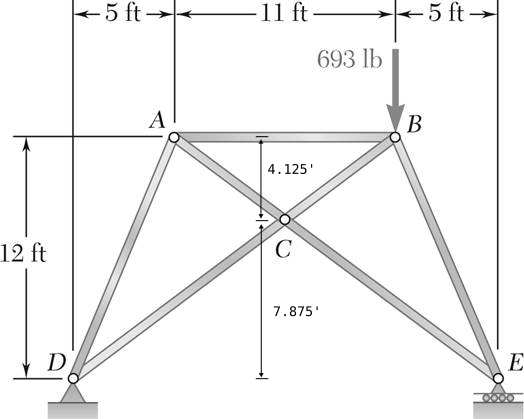
\includegraphics[width=0.5\textwidth,
	           height=0.4\textheight,
		   keepaspectratio]{fig-qz.png}
\end{figure*}


